\chapter{Geocentrický přístup}% MARK: Geocentrický přístup
Již \citeauthor{dsh} věděli, že míra orbitální odlišnosti je silně spojena s rozdílem orbitálních energií meteoroidů. \citeauthor{newapproach} tento přístup využili mnohem více; použili idealizovaný model oběhu Země a meteoroidů a orbitální elementy přetransformovali na geocentrickou rychlost a několik alternativních úhlů \cite{newapproach}. Jejich přístup se ukázal býti velmi úspěšným, v \citeauthor{galligan}ově porovnání tato metoda identifikuje meteorické roje s nejméně vyloučenými členy \cite{galligan}.

Metoda v této kapitole popisovaná je založená primárně na geocentrické rychlosti meteoru, kterou již ze sekce \ref{sec:photography} umíme (alespoň u fotografických pozorování) získat. Výhodou je, že narozdíl od předchozích měr orbitální odlišnosti pro tuto následující míru potřebujeme znát pouze geocentrickou rychlost, rektascenzi a deklinaci meteoru \cite{newapproach}. 

\section{Semi-invariantní orbitální veličiny}% MARK: Semi-invariantní orbitální veličiny
S každým obíhajícím tělesem se pojí několik veličin, které se v čase buďto vůbec nemění, nebo se na dlouhých časových škálách \textit{téměř} nemění. Vzhledem ke gravitačnímů působení všech velkých těles ve Sluneční soustavě nemůžeme považovat elementy dráhy za dlouhodobě konstantní, je ale známo několik parametrů, například geocentrická rychlost, které sice krátkodobě oscilují, ale v řádech tisíců let zůstávají prakticky konstantní \cite{newapproach}: Tyto veličiny nazýváme \textit{sekulárními semi-invarianty}.

\medskip

Pro zavedení několika z nich předpokládejme, že Země obíhá po kruhové dráze na rovině ekliptiky ve vzdálenosti $1$. Také gravitační konstantu, hmotnost Slunce a heliocentrickou rychlost Země položme rovny $1$. Pro nehmotný meteoroid se známými elementy dráhy pak zavádíme \textit{Tisserandův parametr} \cite{newapproach}
\begin{equation}
    T=\frac{1}{a}+2\sqrt{a(1-e^2)}\cos{i} \text{,}
\end{equation}
první ze sekulárních semi-invariantů, který nám v těchto jednotkách dává geocentrickou rychlost \cite{newapproach}
\begin{equation}
    U=\sqrt{3-T}\text{.}
\end{equation}

Zvolíme-li geocentrický systém souřadnic s osou $y$ směřující do zemského apexu a osou $z$ kolmou na rovinu ekliptiky směrem na sever a osou $x$ směřující ven od Slunce, můžeme jednotlivé komponenty vektoru $\vec{U}$ vyjádřit z elementů dráhy \cite{newapproach}
\begin{equation}
    \begin{aligned}
        U_x & = U\sin{\theta}\sin{\phi} & =\; & \pm\sqrt{2-\frac{1}{a}-a(1-e^2)}  \\
        U_y & = U\cos{\theta}           & =\; & \sqrt{a(1-e^2)}\cos{i}-1          \\
        U_z & = U\sin{\theta}\cos{\phi} & =\; & \pm\sqrt{a(1-e^2)}\sin{i}\text{.}
    \end{aligned}
\end{equation}
Úhel $\theta$ značí odchylku $\vec{U}$ od osy $y$ a $\phi$ je úhel mezi rovinou $y-z$ a rovinou obsahující $\vec{U}$ a osu $y$ \cite{newapproach}.

Přepočet z elementů dráhy může být též užitečný, nicméně tato geocentrická rychlost může být vypočtena také pouze z geocentrické rychlosti $v_G$, rektascenze $\alpha$ a deklinace $\beta$ meteoru, jejichž určení známe ze sekce \ref{sec:photography} a které předcházejí výpočtu elementů dráhy. Vektor $\vec{U}$ tedy můžeme získat také jako \cite{newapproach}
\begin{equation}
    \begin{pmatrix}
        U_x\\U_y\\U_z
    \end{pmatrix}=\text{R}_z(\lambda)\text{R}_x(\varepsilon)\,\frac{v_G}{29{,}7}\begin{pmatrix}
        -\cos{\delta}\cos{\alpha}\\
        -\cos{\delta}\sin{\alpha}\\
        -\sin{\alpha}
    \end{pmatrix}\text{.}
\end{equation}
Zde $\text{R}_x$ a $\text{R}_z$ jsou matice rotace kolem příslušné osy o ekliptikální délku Země $\lambda$ a úhel mezi rovníkem a ekliptikou $\varepsilon$.

\medskip

Úhel $\theta$ je důležitý, jelikož je jeho kosinus dalším semi-invariantem \cite{newapproach}. Je proto užitečné jej z rovnic výše vyjídřit jako \cite{newapproach}
\begin{equation}
    \cos{\theta}=\frac{1-U^2-1/a}{2U}\text{.}
\end{equation}
Též budeme dále používat úhel $\phi$, ten ovšem nelze vyjádřit lépe než trigonometricky jako \cite{newapproach}
\begin{equation}
    \phi=\arctan{\frac{U_x}{U}}\text{.}
\end{equation}

\medskip

Semi-invarianty $U$ a $\cos{\theta}$ jsou hlavními používanými veličinami v následující míře orbitální odlišnosti. Existují i další, \cite{newapproach} nabízí například \textit{Kozaiův integrál} $K$, jeho výpočet je ovšem obtížný a pro míru není užitečný. Zanedbáme-li navíc možnost blízkých průletů meteoru kolem planet, stanou se semi-invariantními i orbitální energie $E=-\frac{1}{2a}$ a komponenta momentu hybnosti $L_z=\sqrt{a(1-e^2)\cos{i}}$, ze kterých lze také získat Tisserandův parametr $T=2(L_z-E)$ \cite{newapproach}.

\section{Geocentrická funkce $D_\text{N}$}% MARK: Geocentrická funkce DN
\citeauthor{newapproach} nabízejí hned dvě míry orbitální odlišnosti: $D_\text{N}$ a její zjednodušenou formu $D_\text{R}$. Zjednodušená forma je postavena čistě na výše definovaných semi-invariantech a má tvar \cite{newapproach}
\begin{equation}
    D_\text{R}^2(A,B)=\left( U_B-U_A \right)^2+w_1\left( \cos{\theta_B} - \cos{\theta_A} \right)^2\text{,}
\end{equation}
kde $w_1$ je libovolná váha, obvykle se ale používá a postačuje volba $w_1=1$ \cite{newapproach}\cite{galligan}.

Díky použití sekulárních semi-invariantů je tato metoda také velmi stabilní v čase, na rozdíl od např. $D_\text{SH}$, která, jelikož staví pouze na v čase proměnných elementech dráhy, na dlouhých časových škálách selhává. Porovnání časového vývoje $D_\text{R}$ a $D_\text{SH}$ ukazuje obrázek \ref{img:new:time}.

\begin{figure}[ht]
    \centering
    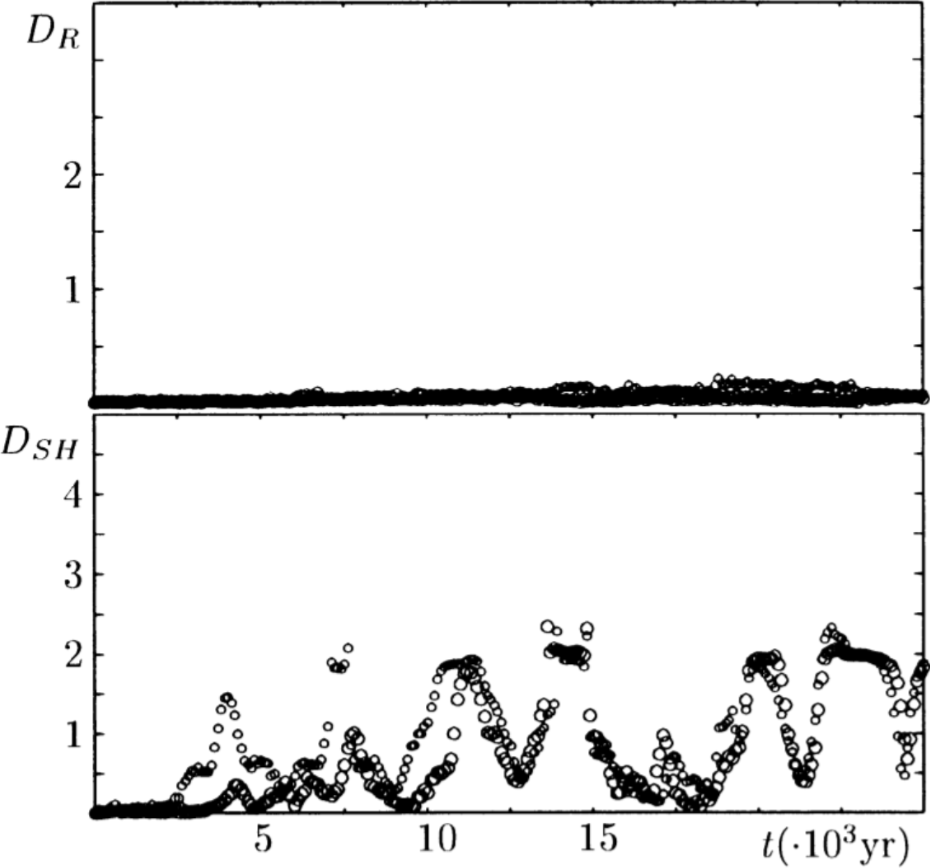
\includegraphics[width=0.5\linewidth]{img/newapproach-time-evolution.png}
    \caption[Porovnání časového vývoje hodnot funkcí $D_\text{R}$ a $D_\text{SH}$]{
        Porovnání časového vývoje hodnot funkcí $D_\text{R}$ a $D_\text{SH}$\\
        {\small (zdroj: \cite{newapproach})}
    }
    \label{img:new:time}
\end{figure}

\medskip

Kompletní kritérium má předpis \cite{newapproach}
\begin{equation}
    D_\text{N}^2(A,B)=\left( U_B - U_A \right)^2 + w_1\left( \cos{\theta_B} - \cos{\theta_A} \right)^2 + \Delta\xi^2 \text{,}
\end{equation}
kde
\begin{eqnarray}
    \Delta\xi^2 &=& \min{\left\{ \left( w_2\Delta\phi_\text{I}^2 + w_3\Delta\lambda_\text{I}^2 \right),\;
                                 \left( w_2\Delta\phi_\text{II}^2 + w_3\Delta\lambda_\text{II}^2 \right) \right\}} \text{,}\\
    \Delta\phi_\text{I} &=& 2\sin{\frac{\phi_B-\phi_A}{2}} \text{,}\\
    \Delta\phi_\text{II} &=& 2\sin{\frac{180^\circ+\phi_2-\phi_1}{2}} \text{,}\\
    \Delta\lambda_\text{I} &=& 2\sin{\frac{\lambda_B-\lambda_A}{2}} \text{ a konečně}\\
    \Delta\lambda_\text{II} &=& 2\sin{\frac{180^\circ+\lambda_B-\lambda_A}{2}} \text{.}
\end{eqnarray}
$\lambda$ je zde ekliptikální délka Země v okamžiku pozorování daného meteoru a $w_2$ a $w_3$ jsou opět volitelné váhy, které se obvykle nastavují na jedničku.

Jako vhodné hranice pro kritérium $D_\text{N}$ určil \citeauthor{galligan} hodnoty \cite{galligan}
$$
    D_\text{N} \le \begin{cases}
        0{,}08 & i < 10^\circ \\
        0{,}09 & 10^\circ \le i < 90^\circ \\
        0{,}17 & i \ge 90^\circ \text{.}
    \end{cases}
$$